\documentclass[12pt]{article}
\usepackage{datetime}
\usepackage{acronym}
\usepackage{xcolor}
\setlength {\marginparwidth }{2cm}
\usepackage{todonotes}
\usepackage{hyperref}
\usepackage{amsmath}
\usepackage{subcaption}
\usepackage{tikz}
\usetikzlibrary{arrows,shapes.geometric,positioning,automata,calc}
% \usepackage{textcomp}
% \usepackage{mathrsfs}  % mathscr font
% \usepackage[colorlinks, filecolor=dark_blue, urlcolor=dark_blue, linkcolor=black, citecolor=black]{hyperref}

\usepackage[
	backend=biber,
	sorting=none,
]{biblatex}
\addbibresource{bibliography.bib}
\usepackage{cleveref}

\newcommand{\meta}[1]{{\color{blue}#1}}  

\newdateformat{monthyeardate}{\monthname[\THEMONTH], \THEYEAR}

\acrodef{iot}[IoT]{Internet of Things}
\acrodef{cps}[CPS]{Cyber-Physical System}
\acrodef{ac}[AC]{Aggregate Computing}
\acrodef{qos}[QoS]{Quality of Service}
\acrodef{cas}[CAS]{Collective Adaptive Systems}
\acrodef{api}[API]{Application Programming Interface}
\acrodef{iac}[IaC]{Infrastructure as Code}
\acrodef{ci}[CI]{Continuous Integration}
\acrodef{ai}[AI]{Artificial Intelligence}
\acrodef{dl}[DL]{Deep Learning}
\acrodef{wcs}[WCS]{Wearable Computing System}
\acrodef{iac}[IaC]{Infrastructure as Code}
\acrodef{rl}[RL]{Reinforcement Learning}

\begin{document}

\begin{titlepage}
	\centering

	\textsc{\Large Ph.D Programme in Computer Science and Engineering}\\[0.5cm]
	\textsc{\Large Admission XXXIX Cycle}\\[0.6cm]

	\hrule width \hsize \kern 1mm \hrule width \hsize height 2pt
	\vspace{0.8cm}

	{\large \bfseries Research Project Proposal}\\[0.6cm]
	{\large \emph{Engineering Reconfigurable Collective Systems in Cloud-Edge Environments}}\\[0.6cm]

	{\bfseries{\monthyeardate\today} \hfill \bfseries{Nicolas Farabegoli}}\\[0.6cm]

	\hrule width \hsize height 2pt \kern 1mm \hrule width \hsize height 1pt
	\vspace{0.4cm}

	\begin{abstract}
		In recent years,
		the emergence of \ac{cps} has engendered a noteworthy surge in complexity and heterogeneity
		within the underlying infrastructure supporting these systems.
		Notably, the interplay between cloud, fog, and edge computing exemplifies the intricacy inherent in such systems.
		%
		Modern collective adaptive applications like \ac{iot}, human enhanced by wearable devices,
		swarm robotics, smart cities,
		are designed to be executed on several devices and to be deployed in
		heterogeneous infrastructures, ranging from cloud servers to wearable devices.
		%
		The availability of such a wide range of devices and infrastructures opens to
		better exploitation of the available resources and performance,
		but introduces complexity in the design and deployment of such applications.
		%
		This research project proposes to produce a framework for the design and deployment of
		collective adaptive applications on heterogeneous infrastructures.
		%
		Reconfiguration aspects will be considered,
		allowing the application to adapt to the changes in the infrastructure and external conditions.
		%
		The framework will leverage \ac{ai} techniques to manage the complex task of reconfiguration, e.g.,
		the opportunistic balance between performance and energy consumption.
		%
		The framework will also offer modern approaches to manipulating data over the continuum,
		enabling effective management of sensors and actuators, but also making data available for storage and analysis.
	\end{abstract}
\end{titlepage}

\section{State of the Art}\label{sec:state-of-the-art}

\paragraph{Collective Adaptive Systems}
A \ac{cas} is a system composed of several entities that interact with each other and can dynamically adapt to changing environments or requirements~\cite{DBLP:conf/birthday/HolzlW11}.
%
Many modern systems are collective adaptive systems,
like \emph{smart cities}, \emph{collective cyber-physical systems}, \emph{robot swarms}, and \emph{sensors network}.

Coordination~\cite{DBLP:journals/csur/Ciancarini96} in \ac{cas} is a fundamental aspect to consider when adaptation properties are required,
and represents an effective way to achieve a global goal in a distributed system.
%
In the literature,
there are several approaches for coordination:
\emph{message passing}~\cite{DBLP:journals/jacm/HondaYC16}, \emph{tuple space models}~\cite{DBLP:books/sp/omicini01/RossiCD01}, \emph{stigmergy models}~\cite{DBLP:journals/cogsr/Heylighen16}.

Situatedness and time awareness are two important aspects of pervasive systems.
%
For this reason,
spatial computing has emerged to manage these aspects as a first-class citizen~\cite{Beal_Viroli_2015}.
%
This approach makes it possible to obtain self-adaptive properties in the system,
and react to changes in the environment and faults conditions.

\ac{ac}~\cite{DBLP:journals/computer/BealPV15} is a novel approach that consists in manipulating computational fields in a declarative and compositional way.
%
This approach shifts the focus from a local perspective to a global one,
where a group of devices can be seen as a single entity in which the aggregate program is executed.

\paragraph{Edge-Cloud Continuum}
\meta{
The Cloud continuum represents one of the most recent hypes in the cloud computing domain with high interest from funding agencies~\cite{ict-40-2020, horizon-cl4-2022-data-01-02}.
%
Even if there is a lot of interest in this topic,
there is no consensus on the definition of the edge-cloud continuum~\cite{DBLP:journals/access/MoreschiniPLNHT22}.
%
The earliest definitions of \emph{Cloud continuum} was proposed in~\cite{DBLP:journals/corr/GuptaNCG16, DBLP:journals/iotj/ChiangZ16} in 2016,
where both focus on the concept of \emph{fog} between cloud and edge to express the concept of the continuum.
%
Over the years, the definition of the Cloud continuum has evolved,
even from the same authors.
%
In~\cite{DBLP:journals/access/MoreschiniPLNHT22} the authors try to organize all the definitions of the Cloud continuum proposed in the literature,
and they find out that there are three main categories: the first one put the concept of ``continuum'' strictly related to the concept of fog.
%
The second one considers the continuum as a combination of multiple edge and fog devices.
%
The third one considers the continuum as a combination of heterogeneous resources spanning from the edge to the cloud.
%
Also, the \ac{iot} is mentioned in the definition of the continuum~\cite{DBLP:conf/ucc/SpillnerGBV20, 9116796},
but it is not clear the relation between \ac{iot} and the continuum.

Moreschini et al. propose a definition that merges two aspects: \emph{extension of the resources} and \emph{extension of computational capabilities}.
%
As a result, they formulate the definition of cloud continuum as \emph{``an extension of the traditional Cloud towards multiple entities (e.g., Edge, Fog, IoT) that provide analysis, processing, storage, and data generation capabilities.''}

What emerges from the literature is that the Cloud continuum is a concept that is still evolving,
but it is quite clear that heterogeneity and complexity in the management of the infrastructures are predominant aspects of the continuum.
%
In this regard,
based on the application context and scenarios,
application-specific approaches are proposed to tackle those complexities~\cite{DBLP:journals/tiot/NehaPSSG22, DBLP:journals/csur/WeisenburgerWS20, DBLP:journals/fi/CasadeiPPVW20},
where each approach has its advantages and disadvantages, but also its application context.
}

\paragraph{Pulverisation}
The deployment of \ac{cas} is a complex task,
especially when the system is composed of a large number of devices.
%
The deployment can also be complicated by the heterogeneity of the devices,
which can have different computational capabilities and different communication technologies, 
and by the dynamicity of the system.
%
Frequently,
in those systems,
the functional aspects are tightly coupled with the deployment aspects,
which makes the deployment of the system rigid and difficult to change.

\emph{Pulverisation}~\cite{DBLP:journals/fi/CasadeiPPVW20} represents an approach to distributed application partitioning and deployment,
where its goal is to provide a way to specify the functional semantics of the software in a deployment-independent way.
%
To do so,
the application logic should be designed considering a logical system,
which is a set of logical devices forming an arbitrary network topology.
%
The application of each logical device is decomposed into an ensemble of components,
representing respectively a set of \emph{sensors},
a set of \emph{actuators},
a \emph{state},
a \emph{communication} component and a \emph{computation} component modeling the behaviour of the device (see~\Cref{fig:pulv}).
%
\begin{figure}[ht]
	\tikzset{-,
		host/.style={rectangle,draw,line width={2pt},inner sep=10pt,
				outer sep=0, minimum height=1.5cm, minimum width=1.8cm, %text height=0.2cm, 
				text depth=0.5cm,
				fill=black!10!white
			},
		node/.style={rectangle,draw,dotted,line width={1pt}, inner sep=2pt,
				fill=blue!20!white,
				font=\large
			},
		nodeA/.style={node,fill=red!20!white},
		nodeB/.style={node,fill=green!20!white},
		nodeC/.style={node,fill=black!30!white},
		nodeD/.style={node,fill=white!20!white},
		plink/.style={line width=2pt},
		llink/.style={dotted,line width=2pt,red},
		hostThin/.style={rectangle,draw,line width={0.5pt},inner sep=10pt,
				outer sep=0, minimum height=1.1cm, minimum width=1.8cm, %text height=0.2cm, 
				text depth=0.5cm,
				fill=black!10!white
			},
		lnode/.style={node,minimum width=0.55cm,minimum height=0.55cm},
		loglink/.style={->,line width=1.5pt}
	}
	\def\nm{0.35cm} %nm = node margin offset
	\def\tpscale{0.7}
	\newcommand{\agent}{device}
	\newcommand{\LSens}{\boldsymbol{\sigma}}
	\newcommand{\LComp}{\boldsymbol{\beta}}
	\newcommand{\LComm}{\boldsymbol{\chi}}
	\newcommand{\LAct}{\boldsymbol{\alpha}}
	\newcommand{\LState}{\boldsymbol{\kappa}}

	\begin{minipage}{\columnwidth}
		\centering
		\begin{tikzpicture}[every node/.style={scale=0.85}]
			\node[hostThin,minimum width=3.4cm,minimum height=3cm,dashed]
			(h1) [label={[yshift=0.35cm]above:{\textbf{logical \agent{}}}}] {};

			\node[lnode] (d1) at (h1.north west) [xshift=\nm,yshift=-\nm,label=above:{behaviour}] {$\LComp$};
			\node[lnode] (d2) at (h1.north east) [xshift=-\nm,yshift=-\nm,label=above:{communication}] {$\LComm$};
			\node[lnode] (d3) at (h1.center) [xshift=0,yshift=0,label=right:{state/knowledge}] {$\LState$};
			\node[lnode] (d4) at (h1.south west) [xshift=\nm,yshift=\nm,label=below:{sensors}] {$\LSens$};
			\node[lnode] (d5) at (h1.south east) [xshift=-\nm,yshift=\nm,label=below:{actuators}] {$\LAct$};

			\node[hostThin,minimum width=2.3cm,minimum height=2.3cm,dashed]
			(h2) [right=2cm of h1, label={above:{\textbf{neighbour \agent{}}}}] {};

			\node[lnode] (d21) at (h2.north west) [xshift=\nm,yshift=-\nm] {$\LComm$};
			\node[lnode] (d22) at (h2.north east) [xshift=-\nm,yshift=-\nm] {$\LComp$};
			\node[lnode] (d23) at (h2.center) [xshift=0,yshift=0] {$\LState$};
			\node[lnode] (d24) at (h2.south west) [xshift=\nm,yshift=\nm] {$\LSens$};
			\node[lnode] (d25) at (h2.south east) [xshift=-\nm,yshift=\nm] {$\LAct$};

			\draw[loglink] (d1) -- (d3);
			\draw[loglink] (d2) -- (d3);
			\draw[loglink] (d3) -- (d1);
			\draw[loglink] (d3) -- (d2);
			\draw[loglink] (d4) -- (d3);
			\draw[loglink] (d3) -- (d5);

			\draw[loglink] (d21) -- (d23);
			\draw[loglink] (d22) -- (d23);
			\draw[loglink] (d23) -- (d21);
			\draw[loglink] (d23) -- (d22);
			\draw[loglink] (d24) -- (d23);
			\draw[loglink] (d23) -- (d25);

			\draw[loglink] (d2.east) -- (d21.west);
			\draw[loglink] (d21.west) -- (d2.east);


		\end{tikzpicture}
		\subcaption{A logical device, split into sub-components, and one of its neighbours.\label{fig:pulv:dev}}
	\end{minipage}
	\\[0.2cm]
	\begin{minipage}{\columnwidth}
		\def\nm{0.3cm} %nm = node margin offset

		\begin{minipage}{0.48\columnwidth}\centering
			\begin{tikzpicture}[node distance=1.0cm and 0.5cm,every node/.style={scale=\tpscale}]
				% physical nodes
				\node[host] (h1) [anchor=north,label=above:{}] {};
				\node[host] (h2) [right=of h1,label=above:{}] {};
				\node[host] (h3) [below=of h1, label=above:{}] {};
				\node[host] (h4) [right=of h3, label=above:{}] {};

				\node[node] (n11) at (h1.south west) [xshift=\nm,yshift=\nm] {$\LSens$};
				\node[node] (n12) at (h1.south east) [xshift=-\nm,yshift=\nm] {$\LComm$};
				\node[node] (n13) at (h1.north east) [xshift=-\nm,yshift=-\nm] {$\LAct$};
				\node[node] (n14) at (h1.north west) [xshift=\nm,yshift=-\nm] {$\LComp$};
				\node[node] (n15) at (h1) [] {$\LState$};
				% logical node 2
				\node[nodeA] (n21) at (h2.south west) [xshift=\nm,yshift=\nm] {$\LComm$};
				\node[nodeA] (n22) at (h2.south east) [xshift=-\nm,yshift=\nm] {$\LAct$};
				\node[nodeA] (n23) at (h2.north east) [xshift=-\nm,yshift=-\nm] {$\LSens$};
				\node[nodeA] (n24) at (h2.north west) [xshift=\nm,yshift=-\nm] {$\LComp$};
				\node[nodeA] (n25) at (h2) [] {$\LState$};
				% logical node 3
				\node[nodeB] (n31) at (h3.south west) [xshift=\nm,yshift=\nm] {$\LSens$};
				\node[nodeB] (n32) at (h3.south east) [xshift=-\nm,yshift=\nm] {$\LAct$};
				\node[nodeB] (n33) at (h3.north east) [xshift=-\nm,yshift=-\nm] {$\LComm$};
				\node[nodeB] (n34) at (h3.north west) [xshift=\nm,yshift=-\nm] {$\LComp$};
				\node[nodeB] (n35) at (h3) [] {$\LState$};
				% logical node 4
				\node[nodeC] (n41) at (h4.south west) [xshift=\nm,yshift=\nm] {$\LSens$};
				\node[nodeC] (n42) at (h4.south east) [xshift=-\nm,yshift=\nm] {$\LAct$};
				\node[nodeC] (n43) at (h4.north east) [xshift=-\nm,yshift=-\nm] {$\LComp$};
				\node[nodeC] (n44) at (h4.north west) [xshift=\nm,yshift=-\nm] {$\LComm$};
				\node[nodeC] (n45) at (h4) [] {$\LState$};

				% physical links
				\draw[plink]
				(h1) -- (h2)
				(h2) -- (h3)
				(h2) -- (h4)
				(h3) -- (h4)
				;
				% logical links
				\draw[llink]
				(n12) to [] (n21)
				(n21) to [] (n44)
				(n21) to [bend right=30] (n33)
				(n33) to [] (n44);
			\end{tikzpicture}
			\subcaption{Peer-to-peer architecture: one-to-one mapping between logical and physical devices, with no offloading.\label{fig:pulv:p2p}}
		\end{minipage}
		\hfill
		\begin{minipage}{0.48\columnwidth}\centering
			\begin{tikzpicture}[node distance=1.0cm and 0.5cm,
					every node/.style={scale=0.6}]

				% physical nodes
				\node[hostThin,minimum width=1.5cm] (h1) [anchor=north,label=above:{}] {};
				\node[hostThin,minimum width=1.5cm] (h2) [right=of h1,label=above:{}] {};
				\node[hostThin,minimum width=1.5cm] (h3) [right=of h2, label=above:{}] {};
				\node[host,minimum width=2.5cm] (he) [above right=0.6cm and -1cm of h1,label=above:{}] {};
				\node[host,minimum width=3.5cm] (h5) [above=2.6cm of h2,label=right:{}] {};

				\node[node] (n11) at (h1.south west) [xshift=\nm,yshift=\nm] {$\LSens$};
				\node[node] (n12) at (h1.south east) [xshift=-\nm,yshift=\nm] {$\LAct$};
				\node[node] (n13) at (he.south east) [xshift=-4*\nm,yshift=\nm] {$\LComm$};
				\node[node] (n14) at (he.south west) [xshift=1*\nm,yshift=\nm] {$\LComp$};
				\node[node] (n15) at (he.north) [xshift=-2*\nm,yshift=-\nm] {$\LState$};
				% logical node 2
				\node[nodeA] (n21) at (h2.south west) [xshift=\nm,yshift=\nm] {$\LSens$};
				\node[nodeA] (n22) at (h2.south east) [xshift=-\nm,yshift=\nm] {$\LAct$};
				\node[nodeA] (n23) at (he.south east) [xshift=-2.5*\nm,yshift=\nm] {$\LComm$};
				\node[nodeA] (n24) at (he.south west) [xshift=2.5*\nm,yshift=\nm] {$\LComp$};
				\node[nodeA] (n25) at (he.north) [xshift=0,yshift=-\nm] {$\LState$};
				% logical node 3
				\node[nodeB] (n31) at (h3.south west) [xshift=\nm,yshift=\nm] {$\LSens$};
				\node[nodeB] (n32) at (h3.south east) [xshift=-\nm,yshift=\nm] {$\LAct$};
				\node[nodeB] (n33) at (h5.south east) [xshift=-5*\nm,yshift=\nm] {$\LComm$};
				\node[nodeB] (n34) at (h5.south east) [xshift=-3*\nm,yshift=\nm] {$\LComp$};
				\node[nodeB] (n35) at (h5.south east) [xshift=-1*\nm,yshift=\nm] {$\LState$};

				% physical links
				\draw[plink]
				(h1) -- (he)
				(h2) -- (he)
				(h3) -- (h5)
				(he) -- (h5);

				\draw[llink]
				(n23) to [bend left=25] (n33);
			\end{tikzpicture}
			\subcaption{IoT hosts can be thin, with some components offloaded at the edge and cloud.\label{fig:pulv:full}}
		\end{minipage}
	\end{minipage}

	\caption{Pulverisation model and examples of deployments (Figure from~\cite{DBLP:journals/fi/CasadeiPPVW20}).}
	\label{fig:pulv}
\end{figure}
%
Decomposition of an application via pulverisation can be achieved in two ways:
either the application is designed with pulverization in mind,
or the application is developed using a framework supporting automatic decomposition such as \ac{ac} frameworks.
%
Once the application is pulverized,
a mapping must be provided between the logical system and the available infrastructure.
%
In this way,
a single logical device (more specifically, its components) can be executed on multiple physical devices,
and a single physical device (host device constituting the infrastructure) can execute multiple logical device components.
%
Moreover,
with no changes,
the application can be deployed on different infrastructures,
without the need to rewrite the application logic.
%
Even if the idea behind pulverisation is quite simple,
several challenges at different levels must be addressed to make it a reality:
\emph{communication}, \emph{portability}, \emph{runtime} are only some of them.


\newpage

% --------------------
% Project description
% --------------------

\section{Project description}\label{sec:project-description}
\meta{
With this project,
we aim to investigate new developing models,
architectures,
and engineering tools for \ac{cas}.
%
Specifically,
this project can be framed on the \emph{COMMunity-OrieNted WEARable Computing Systems} (COMMON-WEARS)~\footnote{\url{https://common-wears.github.io/2022/project/}} project.

The COMMON-WEARS project aims to develop a new generation of wearable computing systems that are community-oriented,
featuring multi-user collectives of smart wearables and body sensor networks (BSN),
with many potential applications like smart cities,
healthcare,
emergency,
and manufacturing, for citing a few.

The development of new models and architecture for next-generation of community-oriented wearable computing systems,
the definition of rigorous engineering methodologies,
simulation tools and formal verification to support the design and development of such systems,
are a few of the main objectives of the COMMON-WEARS project.

Based on the objective stated above,
this project tries to contribute in the following three main directions:

\begin{itemize}
	\item Leverage the \emph{pulverisation} approach for the deployment of \ac{cas} for wearable computing systems.
		In particular,
		we aim to extend the pulverization model to support \textbf{dynamic reconfiguration} of the system,
		to better cope with the dynamicity of the environment and the system itself.
		Moreover, \textbf{\ac{ai} techniques} will be investigated to improve the dynamic reconfiguration of the system.

	\item Bridge the gap between the \emph{simulation} and the \emph{deployment} of such systems.
		Simulation tools represent an effective way to evaluate the system before its deployment,
		however,
		the transition from simulation to deployment is not always straightforward.
		We aim to provide a \textbf{full-stack solution} to support the transition from simulation to deployment of a system with minimal effort.
		% We aim to design and prototype a \textbf{pulverization framework} which can be integrated with existing simulation tools,
		% allowing the simulation of the pulverized system and its deployment on the target infrastructure with minimal effort.
	
	\item \textbf{Engineering data stream on the continuum}: \emph{edge-cloud continuum} represents a new promising infrastructure for the deployment of \ac{cas},
		but also for systems of wearable devices.
		Engineering data stream produced by sensors to control the actuators over the continuum is a challenging task.
		We aim to investigate methodologies ad techniques to support the engineering of the data stream over the continuum to provide more effective control of distributed actuators,
		and consequently,
		enabling data storage and analysis.
\end{itemize}

The following sections provide more details about the three main contributions of this project,
in particular,
they try to illustrate the main challenges and possible solutions.
}
\subsection{Pulverization with dynamic reconfiguration}\label{sec:pulv-dyn}

\meta{
One current limitation of the \emph{pulverization}~\cite{DBLP:journals/fi/CasadeiPPVW20} approach regards the runtime reconfiguration of the system based on the changing conditions or requirements.
%
This project aims to extend the current pulverisation approach to support the dynamic reconfiguration of the system
by combining two approaches: \emph{Rule-based} and \emph{AI-based reconfiguration}.
%
The former can be used to define a set of static rules that can be used to reconfigure the system based on pre-determined and well-known conditions.
%
The latter can be useful in contexts where the unpredictable conditions can be high,
or where a huge number of factors must be considered to determine the best configuration for the system,
making traditional optimization techniques not suitable.
%
In this case,
the \emph{distributed intelligence} can be exploited from two different perspectives:
\emph{application level} to support application logic,
for example by learning the best policy to follow to achieve a specific goal,
and \emph{infrastructural level} to opportunistically choose the best deployment for the system,
based on the current conditions, requirements, or \ac{qos}.
%
In~\Cref{fig:ai-reconf},
we show an example of application decomposition via pulverization and the dynamic relocation of the component over the continuum.
%
\begin{figure}[ht]
	\centering
	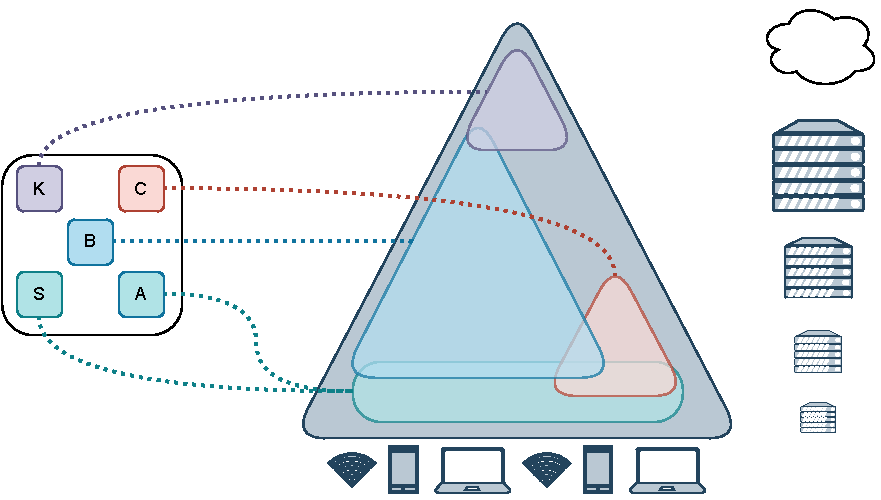
\includegraphics[width=0.55\linewidth]{img/phd-proposal.drawio.pdf}
	\caption{Application decomposition via pulverization and dynamic reconfiguration in the edge-cloud continuum.}
	\label{fig:ai-reconf}
\end{figure}
%
The ability to dynamically reconfiguration is a fundamental aspect,
for example,
in contexts where \emph{energy-efficient} systems are required,
or where the balance between consumption and performance can be strategic.
}

\subsection{Bridge the gap between simulation and deployment}\label{sec:bridge-gap}
\meta{
A the time of writing,
the pulverisation approach has no concrete implementation,
and the validation of the approach has been done via simulations and formal verification~\cite{DBLP:journals/fi/CasadeiPPVW20, DBLP:journals/iotj/CasadeiFPPSV22}.

For this reason,
this project aims to design and prototype a \emph{pulverization framework} that can be used to deploy pulverized applications on the target infrastructure.
%
Moreover,
the integration of the framework with existing simulators like Alchemist~\cite{DBLP:journals/jos/PianiniMV13} is a fundamental step towards the deployment of pulverized applications.
%
As a consequence,
we aim to provide a set of \emph{methodology},
\emph{tools},
and \emph{techniques} that can be seamlessly exploited to effectively engineer \ac{cas} as a full-stack solution.

This contribution can be suitable in scenarios like \emph{smart cities},
\emph{ambient intelligence},
\emph{building automation},
where the unpredictable nature of the environment made it difficult to predict the system's behavior.
%
A full-stack solution can be used to simulate the system before its deployment (and try to predict its behavior),
and then deploy it on the target infrastructure with minimal effort.
}

\subsection{Engineering data stream on the continuum}\label{sec:eng-data-stream}
\meta{
Typically,
in \ac{cps} like \ac{iot} systems or \ac{wcs},
the data are produced at the edge of the network and then manipulated and processed on high-level layers of the network, like the cloud.
%
Taking the pulverization as a reference,
the stream of data produced by the sensors can be manipulated and processed on the continuum,
and then the results can be used to control the actuators (see~\Cref{fig:data-stream}).
%
\begin{figure}[ht]
	\centering
	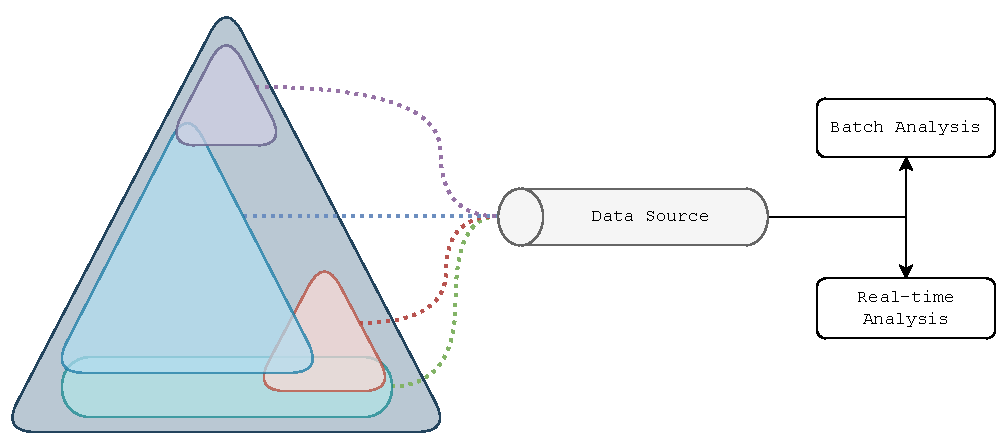
\includegraphics[width=.55\textwidth]{img/data-stream.drawio.pdf}
	\caption{Application decomposition via pulverization and dynamic reconfiguration in the edge-cloud continuum.}
	\label{fig:data-stream}
\end{figure}
%
The effective engineering of the data stream on the continuum is one of the challenges of this project.
%
In particular,
we aim to investigate methodologies and techniques to support the engineering of the data stream over the continuum to provide more effective control of distributed actuators,
and consequently,
enabling data storage and analysis over the stream.
%
Nevertheless,
the main focus remains on the engineering of the data stream,
and not on the data analysis itself,
which can be seen as a consequence of the engineering process where well-known techniques can be used above the stream.
}
% -----------------
% Expected results
% -----------------

\section{Expected results}\label{sec:expected-results}

\paragraph{Pulverisation framework}
Design and prototype an effective framework to support the development of complex systems
via the pulverisation approach.
%
We will provide a modular and extensible framework that can also be integrated with simulation tools
to allow the validation of the system before its deployment.

\paragraph{Dynamic system reconfiguration}
Extend the pulverisation model to support at runtime the dynamic and opportunistic reconfiguration of the components over the continuum.
%
In the first stage,
we will provide a rule-based approach to define the reconfiguration rules.
%
Then,
we will investigate the possibility to adopt \ac{ai} techniques to automatically manage the system reconfiguration at runtime,
and consequently,
to provide a more flexible and adaptive approach.
%
The final expectation is to have implemented both of these two techniques into the pulverisation framework.

\paragraph{Data stream engineering}
\meta{
Integrate into the framework the efficient data stream processing over the continuum and hide to the user the complexity of the underlying infrastructure.
%
In this way,
the user can focus on the application logic and the stream manipulation,
according to the application logic,
will be performed by the framework itself.
%
The framework can also expose APIs to allow the user to perform data storage and data analysis on the stream.
}

\paragraph{Integration with CAS frameworks}
Integrate the proposed framework with other, consolidated \ac{cas} frameworks
to provide a complete full-stack solution for the development and deployment of complex systems,
with the main focus on exploiting edge-cloud infrastructures.
%
\ac{ac} will be used as a possible solution for engineering \ac{cas},
and also as a possible case study for the framework validation.

% --------------------
% Activities
% --------------------

\section{Project activities}\label{sec:activities}

\subsection{First year goals}\label{subsec:first-year-activities}

The first-year goal,
based on the expected results reported in~\Cref{sec:expected-results},
are reported as follows.

\begin{itemize}
	\item Due to the peculiar nature of the pulverization approach,
		the first step will be to investigate the literature about similar approaches adopted for the development of complex distributed systems,
		for example, multi-tier programming and distributed reactive programming for engineering \ac{cas},
		to better understand how these approaches are related to the pulverization approach.
		%
		Then, design and prototype a framework supporting the pulverization approach,
		where modularity and extensibility are the main requirements.
	\item Integrate the framework with a reconfiguration engine to support the dynamic reconfiguration of the system.
	    The reconfiguration engine will be based,
		on a first instance,
		on a rule-based approach allowing the user to specify the conditions in which the system should be reconfigured.
		%
	    The reconfiguration rules can operate at different levels of granularity,
	    from the single device to the entire system.
\end{itemize}

\subsection{PhD goals}\label{subsec:phd-activities}

From~\Cref{sec:expected-results},
the remaining goals of the project are reported as follows.

\begin{itemize}
	\item Contribute to the scientific community with new approaches for the dynamic system reconfiguration based on \ac{ai} techniques.
		In particular,
		we will investigate the use of consolidated and well-known \ac{ai} techniques like \ac{rl},
		to not be used only at application-level,
		but also supporting the system reconfiguration in scenarios where the dynamicity and unpredictability of the environment make difficult the adoption of traditional approaches.
	\item Provide a full-stack solution for engineering \ac{cas}.
		In particular,
		we will investigate the integration of the proposed framework with other consolidate \ac{ac} frameworks like ScaFi~\cite{DBLP:journals/softx/CasadeiVAP22} and Protelis~\cite{DBLP:conf/sac/PianiniVB15}.
		%
		This contribution can be seen as a first step in the direction of effective deployment of \ac{cas},
		opening to the implementation of reference use cases.
	\item Contribute to the research area of the cloud-edge continuum by proposing new approaches to the engineering of the data stream on the continuum.
		Several issues can arise in this context,
		and for this reason,
		we will investigate the state of the art of data stream processing,
		and try to figure out their applicability in different contexts.
		%
		Then,
		contribute by proposing new approaches and solutions to the actual limitations of the state-of-the-art techniques.
\end{itemize}

\subsection{Technology}\label{subsec:technology}
\meta{
Cloud computing is a prominent paradigm for computing resource provisioning,
particularly crucial for the future deployment of IoT and CPS systems.
%
The project focuses on understanding cloud computing and technologies provided by major cloud providers like Google Cloud Platform and Amazon Web Services.
%
Additionally,
it explores the integration of the pulverization framework with Infrastructure as Code (IaC) tools like Terraform~\footnote{\url{https://www.terraform.io/}} and Ansible~\footnote{\url{https://www.ansible.com/}} for effective infrastructure management.
%
To handle the distributed nature of data from IoT and CPS systems,
the project investigates techniques in frameworks like Apache Kafka,
Apache Pulsar,
and Apache Flink.
%
Moreover,
the study delves into distributed technologies such as MOM,
specifically RabbitMQ~\footnote{\url{https://www.rabbitmq.com/}} and ZeroMQ~\footnote{\url{https://zeromq.org/}},
along with microservices patterns for achieving system resilience.
%
The use of Kubernetes~\footnote{\url{https://kubernetes.io/}} as an orchestration tool for managing system deployment and dynamic reconfiguration is also considered.
%
Overall,
the project aims to gain insights into these areas to design and deploy robust collective adaptive applications.
}

\subsection{Long-term contribution}
The initiative proposed in this project aims to tackle the complexity of designing and deploying systems on heterogeneous infrastructures,
where the main focus is on \ac{cas}.
%
Beyond the specific contribution of the project,
which the main focus is on the pulverisation approach,
I expect to contribute to the research community by providing new approaches and solutions to the aforementioned challenges.
%
In particular,
I expect to provide a deep understanding of the role of \ac{cas} in modern scenarios like \emph{smart cities}, \emph{large scale \ac{iot} systems}, and so on,
and providing reference implementations of the proposed approaches.
%
Summing up,
this project can be seen as a groundwork for the creation of systems in the edge-cloud continuum where dynamicity and self-adaptation are key aspects.
%
\ac{ai} and data analysis cover a fundamental role in this context,
enabling a new set of opportunities that this project aims to explore.

\newpage

\printbibliography

\end{document}
